\documentclass[11pt]{article}

\usepackage{apacite}
\usepackage{amsmath,amssymb}
\usepackage{graphicx}
\usepackage{color}
\usepackage{url}
\usepackage{fullpage}
\usepackage{setspace}
\usepackage{booktabs}
\usepackage{multirow}
\usepackage{lingmacros}
\usepackage{caption}
\usepackage{subcaption}

%\newcommand{\url}[1]{$#1$}

\definecolor{Blue}{RGB}{50,50,200}
\newcommand{\blue}[1]{\textcolor{Blue}{#1}}

\definecolor{Red}{RGB}{255,0,0}
\newcommand{\red}[1]{\textcolor{Red}{#1}}
\newcommand{\jd}[1]{\textcolor{Red}{[jd: #1]}} 

\definecolor{Green}{RGB}{50,200,50}
\newcommand{\ndg}[1]{\textcolor{Green}{[ndg: #1]}}  

 \newcommand{\denote}[1]{\mbox{ $[\![ #1 ]\!]$}}


\newcommand{\subsubsubsection}[1]{{\em #1}}
\newcommand{\eref}[1]{(\ref{#1})}
\newcommand{\tableref}[1]{Table \ref{#1}}
\newcommand{\figref}[1]{Figure \ref{#1}}
\newcommand{\appref}[1]{Appendix \ref{#1}}
\newcommand{\sectionref}[1]{Section \ref{#1}}


\title{Over overinformativeness: rational redundant referring expressions}

 
\author{{\large \bf Judith Degen, Caroline Graf, Robert X.D.~Hawkins, Noah D.~Goodman} \\
  \{jdegen,ngoodman\}@stanford.edu\\
  Department of Psychology, 450 Serra Mall \\
  Stanford, CA 94305 USA}

\begin{document}

\maketitle


\begin{abstract}
 

\textbf{Keywords:} 
reference; referring expressions; informativeness; probabilistic pragmatics; experimental pragmatics
\end{abstract}

\section{Introduction}
\label{sec:intro}

Reference to objects is one of the most basic and prevalent uses of language. But how do speakers choose amongst the wealth of referring expressions they have at their disposal? How does a speaker choose whether to refer to an object as \emph{the animal}, \emph{the dog}, \emph{the dalmatian}, or \emph{the big mostly white dalmatian}? The context within which the object occurs  (other non-dogs, other dogs, other dalmatians) plays a large part in determining which features the speaker chooses to include in their utterance  -- speakers aim to be sufficiently informative to uniquely establish reference to the intended object. However, speakers' utterances often exhibit what has been claimed to be \emph{overinformativeness}: referring expressions are often more specific than necessary for establishing unique reference, and they are so in systematic ways. However, providing a unified theory for speakers' systematic patterns of overinformativeness has so far proved elusive.

This paper is concerned with  modeling precisely this choice of referring expression (RE). We restrict ourselves to definite descriptions of the form \emph{the (ADJ}?\emph{)}+ \emph{NOUN}, that is, noun phrases that minimally contain the definite determiner \emph{the} followed by a head noun. In addition, any number of adjectives can occur between the determiner and the noun.\footnote{In contrast, we will \emph{not} provide a treatment of pronominal referring expressions, indefinite descriptions, names, or definite descriptions with post-nominal modification, though we offer some speculative remarks on how the approach outlined here can be applied to these cases. \jd{make sure you actually do this.}} A model of these REs will allow us to unify two domains in language production that have been typically treated as separate, and that have typically been treated as interesting for different reasons: the production of so-called overmodified referring expressions on the one hand, which a lot of literature in language production has been devoted to \cite{bla blabla}; and the production of simple nominal expressions, which has so far mostly received attention in the concepts and categorization literature \cite{bla bla}. In the following, we review some of the key phenomena and puzzles in each of these literatures which have for the most part been treated as unrelated. We then present a model of RE production within the Rational Speech Acts \cite{frank2012} framework, which treats speakers as boundedly rational agents that try to optimize the tradeoff between utterance cost and  informativeness. Our key innovation is to relax the assumption that semantic truth functions are deterministic. \jd{one sentence here that inspires intuition} It is this crucial innovation that allows us to provide a unified explanation for a great number of seemingly disparate phenomena from the modified and nominal RE literature.

\subsection{Production of referring expressions: a case against rational language use?}

How should a cooperative speaker produce referring expressions? Grice, in his seminal work, provided some guidance by formulating his famous conversational maxims, intended as a guide to listeners' expectations about good speaker behavior \cite{grice1975}. His maxim of Quantity, consisting of two parts, requires of speakers to:

\begin{enumerate}
	\item \emph{Quantity-1:} Make your contribution as informative as s required (for the purposes of the exchange).
	\item \emph{Quantity-2:} Do not make your contribution more informative than is required.
\end{enumerate}

That is, speakers should aim to produce neither under- nor overinformative utterances. While much support has been found for the former \cite{lots of people}, speakers seem remarkably happy to systematically violate Quantity-2. In modified referring expressions, they routinely produce modifiers that do not uniquely establish reference (e.g., \emph{the small blue thumbtack} instead of \emph{the small thumbtack} in contexts like \figref{fig:sizesufficient} \cite{bla bla}). In simple nominal expressions, speakers routinely choose to refer to an object with a basic level term even when a superordinate level term would have been sufficient for establishing reference (e.g., \emph{the dog} instead of \emph{the animal} in contexts like \figref{subfig:dogartifacts} \cite{bla bla}).

These observations have posed a challenge for rational accounts of language use (including the Gricean one): why this extra expenditure of useless effort? Why this seeming blindness to the level of informativeness requirement? Many have argued from these observations that speakers are in fact not economical \cite{bla}. Some have derived a built-in preference for referring at the basic level from considerations of \jd{bla} and \jd{bla} \cite{Rosch1976}. Others have argued for salience-driven effects on willingness to overmodify \cite{dutch guys}. In all cases, it is argued that informativeness cannot be the key factor in determining the content of speakers' referring expressions.

Here we revisit this claim and show that systematically relaxing the requirement of a deterministic semantics for referring expressions also systematically changes the informativeness of utterances, in effect leading to a reconceptualization of what have been termed \emph{overinformative referring expressions} as \emph{rationally redundant referring expressions}. We begin by reviewing the phenomena of interest that a revised theory of definite referring expressions should be able to account for. 

\subsection{Modified referring expressions}
\label{sec:modified}

Most of the literature on overinformative referring expressions has been devoted to the use of overinformative modifiers in modified referring expressions. The prevalent observation is that speakers frequently do not include only the minimal modifiers required for establishing unique reference, but often also include redundant modifiers \cite{Pechmann1989, nadig2002,  Maes2004, Engelhardt2006, Arts2011, Koolen2011}. However, not all modifiers are created equal: there are systematic differences in the overmodification patterns observed for size adjectives (e.g., \emph{big, small}), color adjectives (e.g., \emph{blue, red}), material adjectives (e.g., \emph{plastic, wooden}), and many others. Here we review some of the intriguing patterns of overmodification that have plagued that literature, focusing for the most part on size and color.


\begin{figure}
\begin{subfigure}{.5\textwidth}
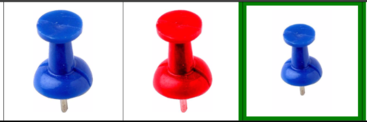
\includegraphics[width=\textwidth]{pics/size-sufficient.png}
\caption{Size sufficient.}
\label{fig:sizesufficient}
\end{subfigure}
\begin{subfigure}{.5\textwidth}
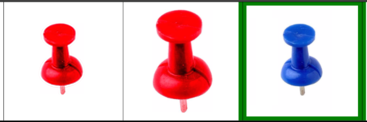
\includegraphics[width=\textwidth]{pics/color-sufficient.png}
\caption{Color sufficient.}
\label{fig:colorsufficient}
\end{subfigure}
\caption{Example contexts where size vs.~color is sufficient for unique reference. A green border marks the intended referent.}
\label{fig:thumbtack}
\end{figure}

\subsubsection{Asymmetry in redundant use of color and size adjectives}
\label{sec:asymmetry}

 In \figref{fig:sizesufficient}, singling out the object with the green border requires only mentioning its size, as in \emph{the small thumbtack}. But it is now well-documented that speakers routinely include redundant color adjectives as in \emph{the small blue thumbtack}, which do not uniquely single out the intended referent in these kinds of contexts \cite{Pechmann1989,  Belke2002, gatt2011}. However, the same is not true for size: in contexts like \figref{fig:colorsufficient}, where color is sufficient for unique reference (\emph{the blue thumbtack}), speakers do not overmodify with size. \tableref{tab:colorsizeasymmetry} shows proportions of color, size, and (overinformative) color-and-size mentions in conditions like those depicted in \figref{fig:thumbtack} across different experiments. In all cases there is a preference for overmodifying with color but not with size.\footnote{There is quite a bit of variation in the actual numbers. We will discuss this variation in the General Discussion. \jd{or already in the model section where we get the basic asymmetry}}
 
 \begin{table}
 \caption{Proportions of color-only, size-only, and color-and-size mentions in color-sufficient vs size-sufficient conditions across experiments.\jd{keep filling in.}}
 	\begin{tabular}{l l l l l l l l}
	\toprule
	 & & \multicolumn{3}{c}{Color sufficient} & \multicolumn{3}{c}{Size sufficient} \\
	Study & Language & Color & Size & Color-and-size & Color & Size & Color-and-size \\
	\midrule
	\citeA{Pechmann1989} & Dutch & 99 & 0 & 1 & 9 & 36 & 55 \\
	\citeA{gatt2011} & English & 92 & 0 & 8 & 3 & 17 & 80\\
 	\citeA{gatt2011} & Dutch & 90 & 0 & 10 & 0 & 21 & 79 \\	
 Our baseline study & English & 94 & 0 & 6 & 2 & 52 & 46 \\ 
	\bottomrule
	\end{tabular}
	\label{tab:colorsizeasymmetry}
 \end{table}

Explanations for this asymmetry have varied. \citeA{Pechmann1989} was the first to take the asymmetry as evidence for speakers following an incremental strategy of object naming: speakers initially start to articulate an adjective denoting a feature that listeners can quickly and easily recognize (i.e., color) before they have fully inspected the display and extracted the sufficient dimension. However, this would predict that speakers routinely should produce expressions like \emph{the blue small thumbtack}, which violate the preference for size adjectives to occur before color adjectives in English. While Pechmann did observe such violations in his dataset, most cases of overmodification did not constitute such violations, and he himself concludes that incrementality cannot (on its own) account for the asymmetry in speakers' propensity for overmodifying with color vs.~size.  

Another explanation for the asymmetry is that speakers try to produce modifiers that denote features that are reasonably easy for the listener to perceive, so that, even when a feature is not fully distinguishing in context, it at least serves to restrict the number of objects that could plausibly be considered the target. Indeed, there has been some support for the idea that overmodification can be beneficial to listeners by facilitating target identification \cite{arts2011, rubiofernandez2016}.

There have been various attempts to capture the color-size asymmetry in computational natural language generation models. The earliest contenders for models of definite referring expressions like the Full Brevity algorithm \cite{Dale1989} or the Greedy algorithm \cite{Dale1989} focused only on discriminatory value -- that is, an utterance's informativeness -- in generating referring expressions, which resulted in an inability to capture the color-size asymmetry: the models only produced the minimally specified expressions. Subsequently, the Incremental algorithm \cite{dale1995} incorporated a preference order on features, with color ranked higher than size. The order is traversed and each encountered feature included in the expression if it serves to exclude at least one further distractor. This results in the production of overinformative color but not size adjectives -- however, the resulting asymmetry is much greater than that evident in human speakers, and is deterministic rather than exhibiting the probabilistic production patterns that human speakers exhibit. More recently, the PRO model \cite{GattEtAl2013} has sought to integrate the observation that speakers seem to have a preference for including color terms with the observation that a preference does not imply the deterministic inclusion of said color term. The model is specifically designed to capture the color-size asymmetry: in a first step, the uniquely distinguishing property (if there is one) is first selected deterministically.  In a second step, an additional property is added probabilistically, depending on both a salience parameter associated with the additional property and a parameter capturing speakers' eagerness to overmodify. If both properties are uniquely distinguishing, a property is selected probabilistically depending on its associated salience parameter. The second step proceeds as before.

However, while the PRO model -- the most state-of-the-art computational model of human production of modified referring expressions -- can capture the color-size asymmetry in and of itself, it is neither flexible enough to be extended straightforwardly to other modifiers beyond color and size, nor can it straightforwardly be extended to capture the more subtle systematicity with which the preference to overmodify with color changes based on various features of context. We delve into these more subtle patterns in the next two sections before presenting our alternative model within the Rational Speech Acts framework.

\subsubsection{Scene variation}
\label{sec:scenevariation}

Speakers' propensity to overmodify with color is highly dependent on features of the distractor objects in the context. In particular, as the variation present in the scene increases, so does the probability of overmodifying with color \cite{Davies2013, Koolen2013}. How exactly scene variation is quantified differs between papers. One very clear demonstration of the scene variation effect was given by \citeA{Koolen2013}, who quantified scene variation as the number of feature dimensions along which objects in a scene vary. Over the course of three experiments, they compared a low-variation condition in which objects never differed in color with a high-variation condition in which objects differed in type, color, orientation, and size. They consistently found higher rates of overmodification with color in the high-variation (28-27\%) than in the low-variation (4-10\%) conditions.

The effect of scene variation on propensity to overmodify has typically been explained as the result of the demands imposed on visual search: in low-variation scenes, it is easier to discern the discriminating dimensions than in high-variation scenes, where it may be easier to simply start naming features of the target that are salient \cite{Koolen2013}. 

\subsubsection{Feature typicality}
\label{sec:colortypicality}

Finally, overmodification with color has been shown to be systematically related to the typicality of the color for the object. Building on work by \citeA{sedivy2003a}, \citeA{Westerbeek2015} (and more recently, \citeA{rubiofernandez2016}) have shown that the more typical a color is for an object, the less likely it is to be mentioned when not necessary for unique reference. For example, speakers never refer to a yellow banana as \emph{the yellow banana}, but they sometimes refer to a brown banana as \emph{the brown banana}, and they almost always refer to a blue banana as \emph{the blue banana}. In fact, color typicality and probability of color mention seem to be negatively correlated in a linear way \cite{Westerbeek2015}. Similar typicality effects have been shown for other (non-color) properties. For example, \citeA{Mitchell2013} showed that speakers are more likely to include an atypical than a typical property (either shape or material) when referring to everyday objects like boxes when mentioning at least one property was necessary for unique reference. %, when the shape and material was atypical (e.g., heart-shaped, made of clay) than when it was typical (e.g., square, made of cardboard). 

Whether speakers are more likely to mention atypical properties over typical properties because they are more salient to \emph{them} or because they are trying to take into account the listener's perspective, for whom presumably these properties are also salient, is an open question \cite{Westerbeek2015}. Some support for the audience design comes from a study by \citeA{Huettig2011}, who found that listeners, after hearing a noun with a diagnostic color (e.g., \emph{frog}), are more likely to fixate objects of that diagnostic color (green), indicating that typical object features are rapidly activated and aid visual search. Nevertheless, the benefit for listeners and the salience for speakers might simply be a happy coincidence and speakers might not, in fact, be designing their utterances for their addressees.

\subsection{Nominal referring expressions}
\label{sec:nominal}

A problem related to the issue of how many additional features to include in a modified referring expression, but which has received much less attention in the language production literature, is that of deciding what taxonomic level to refer to an object to in a simple nominal expression. That is, even in the absence of adjectives, a referring expression can be more or less informative: \emph{the dalmatian} communicates more information about the object in question than \emph{the dog}, which in turn is globally more informative than \emph{the animal}. Thus, this choice can be considered analogous to the choice of adding more modifiers -- in both cases, the speakers has a choice of being more or less specific about the intended referent. However, the choice of reference level in simple nominal referring expressions is also interestingly different from that of adding modifiers in that there is no additional word-level cost associated with being more specific -- the choice is between different one-word utterances, not between utterances of different lengths (in words). 

Nevertheless, cost affects the choice of reference level: in particular, speakers prefer more frequent nouns over less frequent ones \cite{bla}, and they prefer shorter ones over longer ones \cite{bla}. This may go part of the way towards explaining the well-documented effect from the concepts and categorization literature that speakers prefer to refer at the \emph{basic level} \cite{Rosch1976}. That is, in the absence of other constraints, even when a superordinate level term would be sufficient for establishing reference (as in \figref{subfig:dogartifacts}), speakers prefer to say \emph{the dog} rather than \emph{the animal}. However, there are nevertheless cases  of contexts where either the superordinate (\figref{subfig:dogartifacts}) or the basic level (\figref{subfig:doganimals}) term would be sufficient for unique reference, where speakers prefer to use the subordinate level term \emph{the dalmatian} \cite{someone who discusses typicality?}.



\jd{Still not entirely sure what all to discuss here. The generally rich interplay between informativeness, cost, and typicality? Or just focus on the basic level preference?}

\subsection{Summary}
\label{sec:introsummary}

In sum, the production of modified and simple nominal referring expressions is governed by a rich interplay of many factors, including an utterance's informativeness, its cost relative to alternative utterances, and the typicality of an object or its features. We are here especially interested in cases where speakers appear to be overinformative -- either by adding more modifiers or by referring at a more specific level than necessary for establishing unique reference. A summary of the effects we will focus on in the remainder of the paper is provided in \tableref{tab:effects}.

\begin{table}
\caption{List of effects a theory of referring expression production should account for.}
\begin{tabular}{l p{6cm} p{5.5cm} }
\toprule
Effect & Description & Reported by \\
\midrule
Color/size asymmetry & More redundant use of color adjectives than size adjectives &  \citeA{Pechmann1989, Engelhardt2006, gatt2011} \red{others}\\
%Number of distractors & More redundant use of color with increasing number of distractors & ?? \red{deutsch} \\
Scene variation & More redundant use of color adjectives with increasing scene variation & \citeA{davies2009, Koolen2013}\\
Color typicality & More redundant use of color adjectives with decreasing color typicality & \citeA{sedivy2003a, Westerbeek2015, rubiofernandez2016}\\
\midrule
Basic level preference & Preference for basic level term when superordinate level term sufficient & \citeA{Rosch1976} \red{others}\\
Subordinate level mention & Unnecessary use of sub level term when basic or super level sufficient & \red{who?}\\
\red{other??} \\
\bottomrule
\end{tabular}
\label{tab:effects}
\end{table}

To date, there is no theory to account for all of these different phenomena; and no model has attempted to unify overinformativeness in the domain of modified and unmodified referring expressions. We touched on some of the explanations that have been proposed for these phenomena. We also highlighted where computational models have been proposed for individual phenomena, and how they fall short in the grand scheme of things. \jd{make sure you actually review this literature in the preceding sections! ie pro/incremental algorithm/etc}. In the next section, we present the Rational Speech Acts modeling framework, within which we will provide precisely the kind of theory that can account for at least all of the phenomena listed here and holds great promise for scaling up to many other overinformativeness phenomena.  

\section{Modeling speakers' choice of referring expression}
\label{sec:models}

Here we propose an extension to the production component of the Rational Speech Acts \cite<RSA>{frank2012, goodmanstuhlmueller2013} modeling framework that provides a principled explanation for the phenomena reviewed in the previous section, and that holds promise for being generalizable to many further production phenomena related to overinformativeness, which we discuss in the General Discussion. \jd{make a list and make sure to discuss} We proceed by first presenting the general framework in \sectionref{sec:basicrsa}, and show why the most basic model cannot account for any of the phenomena outlined above, due to its strong focus on maximizing the informativeness of one-word expressions under a deterministic semantics. We then show in \sectionref{sec:basiclevelsmodel} how first relaxing the assumption of a deterministic semantics can account for speakers' preferences in the choice of simple nominal referring expressions. We then further extend the model by allowing multi-word utterances; \sectionref{sec:modifiedmodel} shows how this, in combination with the non-deterministic semantics, captures all of the phenomena -- the color-size asymmetry, the scene variation effect, and the color typicality effect -- related to overmodified referring expressions listed in \tableref{tab:effects}.

\jd{Interesting snippet from Pechmann which we should probably quote: ``in information theory, a positive function is assigned to redundancy, since it can compensate for partial loss of information. Can overspecification in referential communication have the same function? We can rule out this possibility, because we regard those utterances as being `redundant' which include nondistinguishing features in addition to distinguishing ones. Yet nondistinguishing features cannot compensate for the loss of distinguishing information, since by definition nondistinguishing features do not distinguish the target referent from context. At best, they can reduce the domain of referential alternatives.'' $\rightarrow$ But that IS compensating!}

\subsection{Basic RSA}
\label{sec:basicrsa}

\jd{introduce the basic model and show why it doesn't get overinformative}

\subsection{RSA with non-deterministic semantics}
\label{sec:basiclevelsmodel}

\jd{standard rsa pragmatic speaker blablabla}





\subsection{Non-deterministic RSA with multi-word utterances}
\label{sec:modifiedmodel}

\red{show the model extension and the predictions it makes for the basic color/size asymmetry. report our replication of gatt?}

\subsection{Number of distractors}
\label{sec:numdistmodel}

The extended noisy semantics model makes a number of novel predictions for the rate of redundant adjective use. In particular, we can ask what the predicted rate of redundant adjective use is as a function of a) the number of distractor items and b) the features of those distractor objects. It has been shown in the past that overmodification increases with the number of distractors that are present \cite{bla}. It has also been established that there is more overmodification in polychrome rather than monochrome displays \cite{bla -- see paula's paper} and in scenes in which objects differ along more feature dimensions \cite{koolen bla}. \red{or save the scene variation stuff for the next section?}

The noisy semantics model's predictions are shown in \figref{fig:numdistractors}. \red{spell out the different conditions and why they're interesting -- why not just number of distractors, why TYPE as well?}

\begin{figure}
\label{fig:numdistractors}
\end{figure}

To test the model's predictions, we conducted two interactive web-based written production studies within a reference game setting.\footnote{See \appref{app:replication}  for a validation of the general paradigm, in which we qualitatively replicate the findings of \citeA{gatt2011} with a different set of stimuli.} Speakers and listeners were shown arrays of objects of that could vary in color and size. Speakers were to produce a referring expression to allow the listener to identify a target object. We manipulated the number of distractor objects in the grid, as well as the variation in color and size among distractor objects.

\subsubsection{Method}

\paragraph{Participants}

We recruited 60 pairs of participants (120 participants total) over Amazon's Mechanical Turk who were each paid \$1.75 for their participation. Here and in all other experiments reported in this paper, participants� IP address was limited to US addresses only and only participants with a past work approval rate of at least 95\% were accepted. The data of five pairs were excluded from analysis because one of the participants dropped out before completing the experiment.

\paragraph{Procedure}

Participants were paired up via \red{is there something in robert's tools to cite?}. For each pair, one participant was assigned the speaker role and one the listener role. They  initially received written instructions \red{more info}. Before continuing to the experiment, participants were required to correctly answer a series of questions about the experimental procedure. These questions are listed in \appref{app:numdistractors}.

On each trial participants saw an array of objects. The array contained the same objects for both speaker and listener, but the order of objects was randomized and was typically different for speaker and listener. In the speaker's display, one of the objects -- henceforth the \emph{target} -- was highlighted with a green border. See \figref{fig:exampledisplay} for an example of the listener's and speaker's view on a particular trial.

\begin{figure}
\label{fig:exampledisplay}
\red{insert example display}
\end{figure}

The speaker produced a referring expression to communicate the target to the listener by typing in a chat window. After pressing Enter or clicking the `Send' button, the speaker's message was shown to the listener. The listener then clicked on the object they thought was the target, given the speaker's message.  Once the listener clicked an object, a red border appeared around that object in both the listener and the speaker's display for 1 second before advancing to the next trial.

Both speakers and listeners could write in the chat window, allowing listeners to request clarification if necessary. Listeners could only click on an object and advance to the next trial once the speaker had sent a message. 

\begin{figure}
\begin{subfigure}{\textwidth}
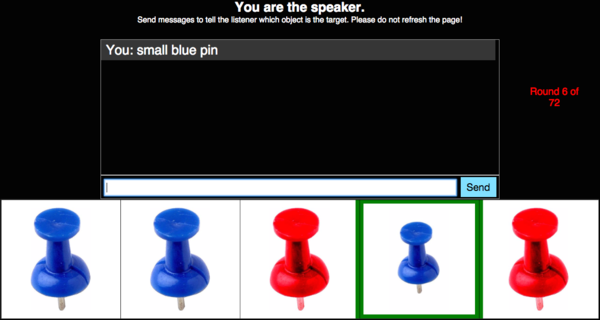
\includegraphics[width=\textwidth]{pics/speaker-perspective-small.png}
\caption{Speakers' perspective}
\label{fig:speakerpersp}
\end{subfigure}

\begin{subfigure}{\textwidth}
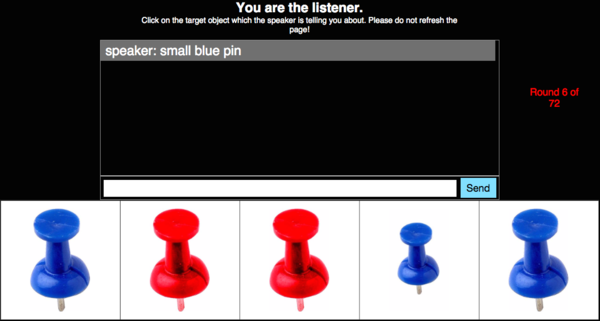
\includegraphics[width=\textwidth]{pics/listener-perspective-small.png}
\caption{Listeners' perspective.}
\label{fig:listenerpersp}
\end{subfigure}
\caption{Example displays from the  (a) speaker's and the  (b)  listener's perspective on a \emph{size-sufficient 4-2} trial.}
\label{fig:speakerlistenerperspective}
\end{figure}

\paragraph{Materials}

Participants proceeded through 72 trials. Of these, half were critical trials of interest and half were filler trials. On critical trials, we varied the feature that was sufficient to mention for uniquely establishing reference, the total number of objects in the array, and  the number of objects that shared the non-sufficient feature with the target. 

Objects varied in color and size. On 18 trials, color was a sufficient property for distinguishing the target. On the other 18 trials, size was sufficient. See \figref{fig:speakerlistenerperspective} for an example of a size-sufficient trial from both the speaker's and the listener's perspective. 


In Exp.~1, the number of distractor objects in each array was either 2 (12 trials) or 4 (24 trials). In Exp.~2, the number of distractor objects in each array was either 2, 3, or 4. Finally, we varied the number of distractors that shared the non-sufficient property with the target. That is, when size was the sufficiently distinguishing property, we varied the number of distractors that shared the same color as the target. This number had to be at least one, since otherwise the non-sufficient property would have been sufficient for uniquely establishing reference, i.e.~it would not have been redundant to mention it. 

In Exp.~1, each total number of distractors (2, 4) was crossed with each possible number of distractors that shared the non-sufficient property, leading to the following six conditions: \emph{2-1, 2-2, 4-1, 4-2, 4-3,} and \emph{4-4}, where the first number indicates the total number and the second number the shared number of distractors. Exp.~2 was conducted in order to additionally collect data for the \emph{3-X} conditions. To this end, Exp.~2 included the \emph{3-1, 3-2}, and \emph{3-3} conditions, as well as three conditions repeated from Exp.~1, in order to ensure that results were comparable. The repeated conditions were \emph{2-1, 4-1}, and \emph{4-3}. An overview of the number of trials in each condition and experiment is provided in \tableref{tab:conditions}.

\begin{table}
\caption{Number of trials in each condition.}
\centering
	\begin{tabular}{c c c c}
	\toprule
	Distractors & Feature-sharing distractors & Trials & Exp.\\
	\midrule
	2 & 1 & 12 & 1 \& 2\\
	2 & 2 & 6 & 1\\
	\midrule
	3 & 1 & 6 & 2\\
	3 & 2 & 6 & 2\\
	3 & 3 & 6 & 2\\
	\midrule
	4 & 1 & 12 & 1 \& 2\\
	4 & 2 & 6 & 1\\
	4 & 3 & 12 & 1 \& 2\\
	4 & 4 & 6 & 1\\			
	\bottomrule
	\end{tabular}
\label{tab:conditions}	
\end{table}

Fillers were target trials from a different experiment \cite{graf-underreview}. Each filler item contained a three-object grid. None of the filler objects occurred on target trials. Objects stood in various taxonomic relations to each other and required neither size nor color mention for unique reference. For example, a filler trial could consist of a display with a dalmatian, a pug, and a squirrel.



\subsubsection{Results}

\begin{figure}
\centering
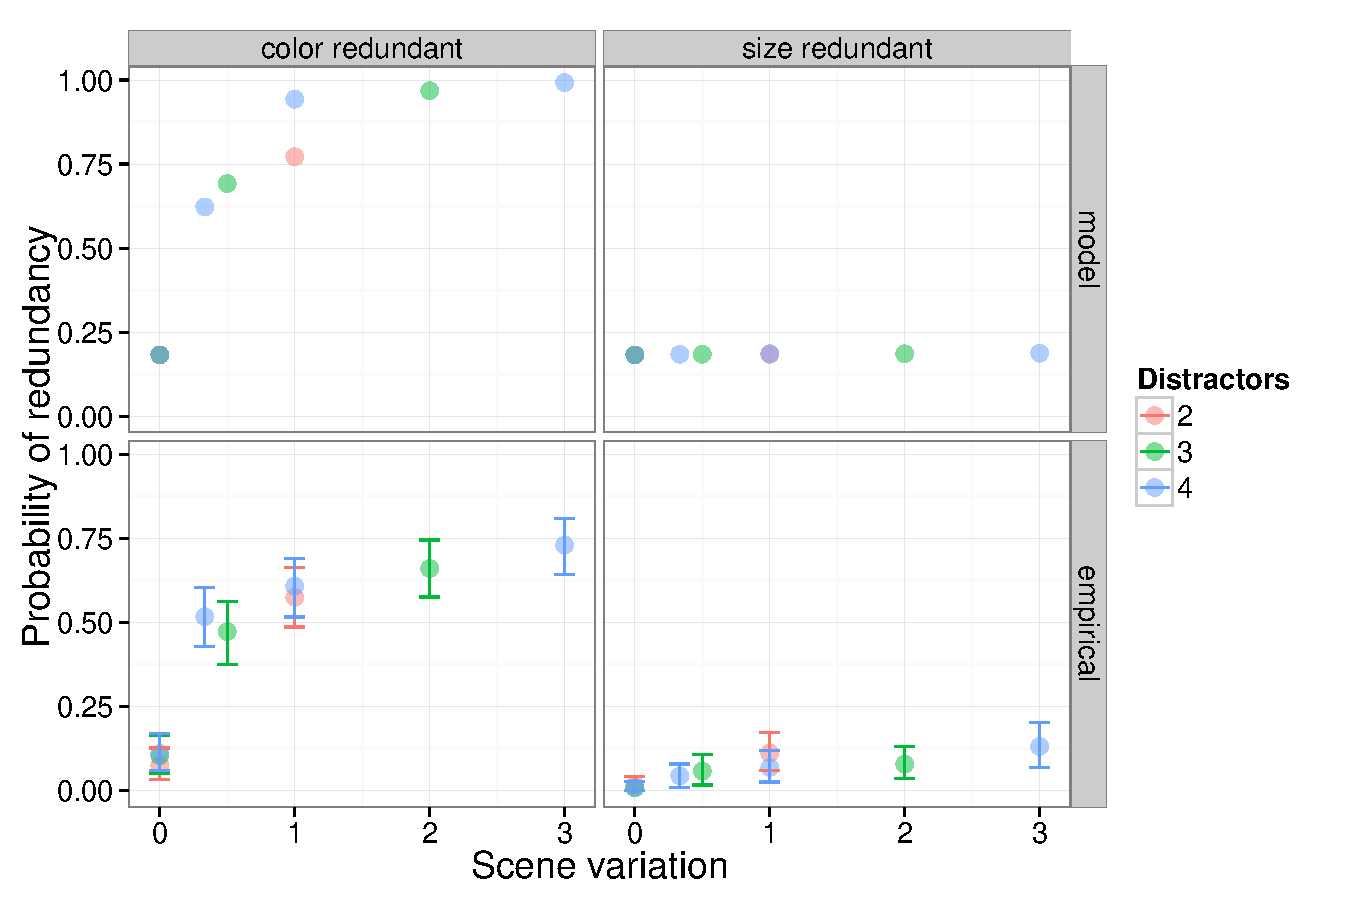
\includegraphics[width=\textwidth]{pics/model-empirical}
\caption{Model predicted probability of redundancy (first column) alongside empirical proportions of redundant descriptions (second column) as a function of the ratio of the number of distractors that differ from the target along the non-sufficient dimension to the number of distractors that do not. Rows indicate the redundant feature. \red{Model params: fcolor .999, fsize .8, lambda 15, costs .1}}
\label{fig:modelexpresults}
\end{figure}

\subsection{Scene variation}
\label{sec:scenevarmodel}

\red{show model predictions for koolen et al scenes -- qualitative effect}

\subsection{Color typicality}
\label{sec:colortypmodel}

\red{set up model extension to get color typicality effect (or will you end up reporting this model from the start?)}

\section{General Discussion}
\label{sec:gd}

\begin{itemize}
	\item talk about how the approach applies to other referring expressions like those mentioned in the intro (indefinite, post-nominal modification pronouns)
	\item talk about how our approach fits in with incremental stories of overspecification?
	\item The work reported here clearly shows that overmodified referring expressions, contrary to some claims in the literature \cite{Engelhardt2011} \red{who say overmodification ipmairs comprehension}, contribute more utility than `minimally' specified referring expressions.
\end{itemize}

\appendix

\section{Validation of interactive web-based written production paradigm}
\label{app:replication}

\red{make sure to discuss why overall we have lower overspecification rates -- probably because of color typicality!! we had pretty typical colors in our stimuli}

\section{Pre-experiment quiz}
\label{app:numdistractors}

Before continuing to the main experiment, each participant had to correctly respond ``True'' or ``False'' to the following statements. Correct answers are given in parentheses after the statement.

\begin{itemize}
	\item The speaker can click on an object. (False)
	\item The listener wants to click on the object that the speaker is
  telling them about. (True)
  \item  The target is the object which has the red circle around it. (False)
  \item Only the speaker can send messages. (False)
  \item There are a total of 72 rounds. (True)
  \item The locations of the three objects are the same for the speaker and the listener. (False)
\end{itemize}



\red{report Gatt et al 2011 replication}

\bibliographystyle{apacite}

\setlength{\bibleftmargin}{.125in}
\setlength{\bibindent}{-\bibleftmargin}

\bibliography{bibs}


\end{document}
